\subsubsection{CAN Protocol description}
A Peak-CAN adapter were used throughout the project. It supports High-speed ISO 11898-2\footnote{\url{http://www.peak-system.com/PCAN-USB.199.0.html?&L=1}} which is a standard that states the properties of physical layer. 
Its max speed is 1 mbit which is the speed AQ uses to communicate on the CAN-bus. 
AQ uses CAN 2.0B which has 29 identifier bits.
AQ is not using an existing protocol on the application layer. The developers created their own to suit their needs.\\

\subsubsection*{Identifier bits}
A Generic look at a AQ CAN messages can be seen in table \ref{tab:can_identifier_bits}.
The normal function of the identifier bits is the priority of the messages.
A CAN controller can then be setup to only allow certain messages to be processed depending on their identifier bits.
The identification bits has been split up in AQ to contain information about the sender, receiver etc. Which is not normally saved information in a CAN message.
\begin{table}[H]
\resizebox{\textwidth}{!}{%
	\begin{tabular}{|c|c|c|c|c|c|c|c|}
	\hline
	\multicolumn{8}{|c|}{CAN Message} \\ 
	\hline
	 \multicolumn{7}{|c|}{Identfier bits [29 bits]} &  		\multicolumn{1}{c|}{Data bits [max 64 bits]} \\
	 \hline
	 LCC [28:27] & TT [26] & FID [25:22] & DOC [21:16] & SOID 	[15:11] & TID [10:16] & SEID [5:0] & \\
	\hline
\end{tabular}}
	\caption{Table shows the identifier bits used in AutoQuad CAN messages}
	\label{tab:can_identifier_bits}
\end{table}

In figure \ref{tab:abbri_can_msg} the abbreviations can be seen.
\begin{table}[H]
		\begin{tabular}{|l|l|}
		\hline
		LCC & Logical Communications Channe \\
\hline
		TT & Target Type \\
\hline
		FID & Function ID \\
\hline
		DOC & Data Object Code \\
\hline
		SOID & Source ID \\
\hline
		TID & Target ID \\
\hline
		SEID & Sequence ID \\
\hline
		\end{tabular}
		\caption{Table shows 
abbreviations used in table \ref{tab:can_identifier_bits}}
		\label{tab:abbri_can_msg}
\end{table}

Each of the elements in an AQ messages will be explained how they are used in AQ. \\

\subsubsection*{Logic Communication Channel}
LCC is the priority of the message. 
To understand how LCC works, one needs to look into CAN arbitration.
As stated in ISO-11898-2, a 0 is the dominant bit and a 1 is the recessive bit.
The example in figure \ref{tab:can_arbitration} shows two nodes each transmitting a packet.
The arbitration only happens during the transmission of the identifier bits.
In the example on bit 8, Node 16 losses the arbitration and stops transmitting.
Node 15 keeps transmitting its packet because it has lower identifier bits and thereby higher priority.
\begin{figure}[H]
    \center
    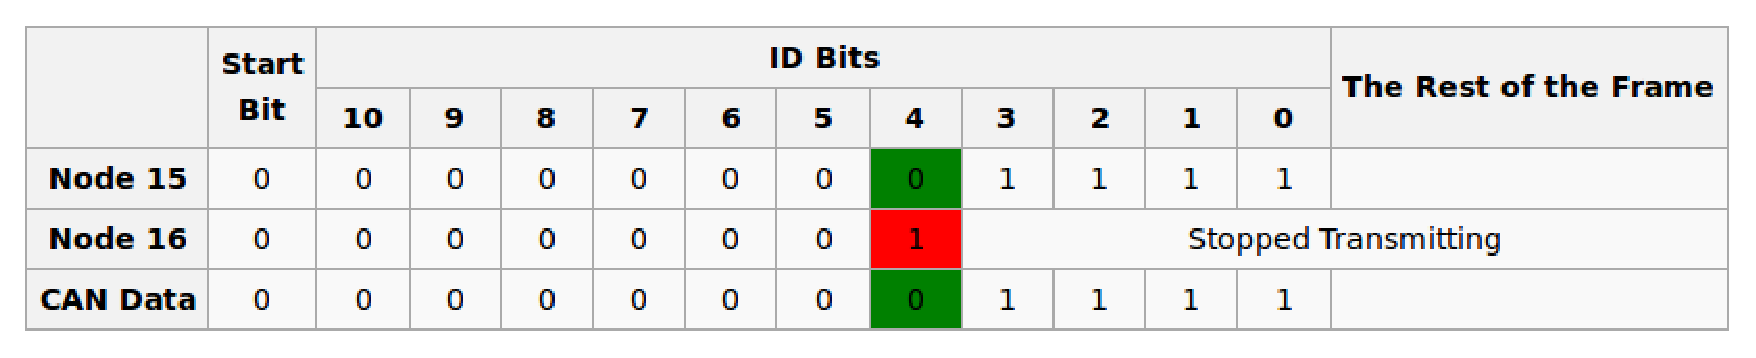
\includegraphics[width=1\textwidth]{graphics/can_arbitration.eps}
    \caption{Example of CAN arbitration where node 15 has the lowest ID and thereby highest priority}
    \label{tab:can_arbitration}
\end{figure}
\newpage
LLC in a message can take one of the defines in code \ref{code:llc_defines}
\begin{lstlisting}[language = c, caption = LLC defines, label=code:llc_defines]
#define CAN_LCC_EXCEPTION   ((uint32_t)0x0<<30)
#define CAN_LCC_HIGH        ((uint32_t)0x1<<30)
#define CAN_LCC_NORMAL      ((uint32_t)0x2<<30)
#define CAN_LCC_INFO        ((uint32_t)0x3<<30)
\end{lstlisting}

\begin{table}[H]
\centering
\caption{Table showing the 4 types of priority in AQ}
\label{my-label}
\begin{tabular}{|l|l|l|}
\hline
\textbf{Name} & \textbf{Value} & \textbf{Priority (lowest first)} \\ \hline
EXCEPTION     & 0000           & 0                 \\ \hline
HIGH          & 0001           & 1                 \\ \hline
NORMAL        & 0010           & 2                 \\ \hline
INFO          & 0011           & 3                 \\ \hline
\end{tabular}
\end{table}

\subsubsection*{Target Type}
Target type can either be “node” or “group” depending on if the receiver(s) is one or more nodes. 
\begin{lstlisting}[language = c, caption = Target type defined in AQ, label=code:target_types]
#define CAN_TT_GROUP        ((uint32_t)0x0<<29)
#define CAN_TT_NODE         ((uint32_t)0x1<<29)
\end{lstlisting}
The GROUP is used when AQ sends its reset-msg upon startup.\\
When the authors node sends a sensor-measure to AQ it will be of type CAN\_TT\_NODE.
\subsubsection*{Function ID}

Function ID describes the function of the CAN message. If it is a PING, ACK, NACK, etc.
It simply states the function of packet so the receiver node knows what to do with the message.
Different types of functions can be seen in code \ref{code:function_defines}
\begin{lstlisting}[language = c, caption = Excerpts from AQ's list of function defines, label=code:function_defines]
#define CAN_FID_RESET_BUS		((uint32_t)0x0<<25)
#define CAN_FID_ACK				((uint32_t)0x1<<25)
#define CAN_FID_REQ_ADDR		((uint32_t)0x7<<25)
#define CAN_FID_GRANT_ADDR	((uint32_t)0x8<<25)
#define CAN_FID_CMD           ((uint32_t)0x3<<25)
\end{lstlisting}

Table \ref{tab:fid_descriptions} describes the FIDs shown in listing \ref{code:function_defines}. \\

\Mathias{Dette er forkert, eftersom alle defines er taget fra AQ's can.h så der passer det..}
If a message is if FID CAN\_FID\_CMD, the Data Object code will be used as the command.\\
It should be noted from code \ref{code:function_defines} that the FID's is moved 25 positions to the left but FID is shown in table \ref{tab:can_identifier_bits} is at bits 22:25. 
The offset of three bits is due to the way ARM's CAN registers is implemented. The three initial bits in CAN\_TIxR and CAN\_RIxR (registers used to transmit and receive respectively) \footnote{\url{http://www2.st.com/content/ccc/resource/technical/document/reference_manual/59/b9/ba/7f/11/af/43/d5/CD00171190.pdf/files/CD00171190.pdf/jcr:content/translations/en.CD00171190.pdf:688}} registers are general information about the CAN messages like whether it is extended (Part B.0) or not.
\begin{table}[H]
\centering
\caption{Descriptions of the FIDs mentioned in code \ref{code:function_defines}}
\label{tab:fid_descriptions}
\resizebox{\textwidth}{!}{%
\begin{tabular}{@{}|l|l|@{}}
\toprule
\textbf{FID}          & \textbf{Description}                                                               \\ \midrule
CAN\_FID\_RESET\_BUS  & Message sent by AQ when powered up                                                 \\ \midrule
CAN\_FID\_ACK         & Message sent to AQ when acknowledging a received message                           \\ \midrule
CAN\_FID\_REQ\_ADDR   & Messaged used when a node on the bus tries to register itself as a node on the bus \\ \midrule
CAN\_FID\_GRANT\_ADDR & Messaged sent by AQ when it registers a node as a node on the bus.                 \\ \bottomrule
\end{tabular}
}
\end{table}

Table \ref{tab:fid_descriptions} shows a description of the 4 FIDs used when a node is registered. 

\subsubsection*{Data Object Code}
Data Object code is used as a parameter to the FID. Data Object Code can have different values depending on the fid. Code \ref{code:doc_useage} shows a function using DOC when message FID is CAN\_FID\_CMD.

\begin{lstlisting}[language = c, caption = Snippet of AQ's can.c:365, label=code:doc_useage]
void canProcessCmd(... ,uint8_t doc, ...) {
    switch (doc) {
        case CAN_CMD_STREAM:
        	...
            break;
        case CAN_CMD_TELEM_VALUE:
        	...
            break;
        case CAN_CMD_TELEM_RATE:
        	...
            break;
    }
}
\end{lstlisting}

In section \ref{sec:reg_aq_node} DOC is used by the author to tell which part of the GPS data is getting sent but where FID is CAN\_FID\_TELEM.
\Mathias{Fixe ref til section om GPS spoof}

\subsubsection*{Source/Target/Network ID}
When referred to source/target ID but without respect to either sender or receiver but just a CAN-node, then it is referred to as NetworkId. When a node registers itself in AQ, it gets assigned a NetworkId.

\subsubsection*{Sequence ID}
The sequence id is incremented on transmission of each message. It is used when eg. 
A CAN-node sends a reply to a get-message, it is then including the sequence id of the get-message so AQ knows what it receives a reply for.

\subsubsection*{Data bits}
The data bytes does not have a general definition, it depends on the function id. With some FIDs the data field may contain additional parameters.\\ \\
Eg. When FID is CAN\_FID\_REQ\_ADDR, data has the fields shown in table \ref{tab:packet_from_node}
\begin{table}[H]
\centering
\caption{Packet sent from node when registering in AQ}
\label{tab:packet_from_node}
\begin{tabularx}{0.92\textwidth}{@{}|X|X|X|X|X|X|X|X|@{}}
\toprule
\multicolumn{8}{|c|}{64 bits}                           \\ \midrule
0 & 0 & CanId & CanType & UUID3 & UUID2 & UUID1 & UUID0 \\
\midrule
7 & 6 & 5 & 4 & 3 & 2 & 1 & 0 \\ \bottomrule
\end{tabularx}
\end{table}

\textbf{UUID} is a unique address generated by each node on the bus. In ESC32v2\footnote{\url{https://github.com/bn999/esc32/blob/master/onboard/can.c}} the address is calculated using XXH-hashing algorithm. The algorithm generates a 32 bit hash from a given input value and a salt.
The input to XXH in ESC32v2 is the unique ID that every ARM in the STMF32\footnote{\url{http://www2.st.com/content/ccc/resource/technical/document/reference_manual/59/b9/ba/7f/11/af/43/d5/CD00171190.pdf/files/CD00171190.pdf/jcr:content/translations/en.CD00171190.pdf}}
 family has. Code \ref{code:xxh_canesc32v2} shows how it is implemented in AQ.

\begin{lstlisting}[language = c, caption = Snippet showing UUID generated in ESC32v2, label=code:xxh_canesc32v2]
can.h:20
#define CAN_UUID	0x1FFFF7E8

can.c:753
canData.uuid = XXH32((void *)CAN_UUID, 3*4, 0);
\end{lstlisting}

\textbf{CanType} is the type of the node trying to register. Eq. SENSOR, ESC and SERVO.  \\

\textbf{CanID} is the number of the CanType node trying to register. When an ESC32v2 is trying to register it sends CanId as the ESC number ranging from 1 to the number of ESC's mounted on the drone. The CanID is assign to each ESC manually as part of the configuring.

% redefine the \mess so that \_ works...
\renewcommand{\mess}[4][0]{
  \stepcounter{seqlevel}
  \path
  (#2)+(0,-\theseqlevel*\unitfactor-0.7*\unitfactor) node (mess from) {};
  \addtocounter{seqlevel}{#1}
  \path
  (#4)+(0,-\theseqlevel*\unitfactor-0.7*\unitfactor) node (mess to) {};
  \draw[->,>=angle 60] (mess from) -- (mess to) node[midway, above]
  {#3};
}

\subsubsection*{Registering a node in AQ}\label{sec:reg_aq_node}

When the AQ is starting up, it is transmitting a CAN\_FID\_RESET\_BUS to the bus.
When each CAN-node receives the messages, they send out a CAN\_FID\_REQ\_ADDR message in order to get registered as a node in AQ.
If a node on the bus does not get registered it will not be able to communicate with AQ. \\
When AQ receives an CAN\_FID\_REQ\_ADDR, it sends back a CAN\_FID\_GRANT\_ADDR to tell the node that the registration is successful and to assign the node its networkID.
This id is used later to identify the node when it is transmitting a message or when AQ wants to send out a message to that specific node.
The sequence diagram in figure \ref{fig:protocol_req_node} shows the described sequence.

\begin{figure}[H]
    \center
      \begin{adjustbox}{max width=0.5\textwidth}
	\begin{sequencediagram}
	  \newthread{0.4}{pynode}{ROS-node}
	  \newthread{7}{autoquad}{AutoQuad}

	  \mess[1]{autoquad}{CAN\_FID\_RESET\_BUS}{pynode}

	  \begin{call}[3]{autoquad}{Wait(100ms)}{autoquad}
			\postlevel
			\postlevel
			\mess{pynode}{CAN\_FID\_REQ\_ADDR}{autoquad}
			\postlevel
			\mess{autoquad}{CAN\_FID\_GRANT\_ADDR}{pynode}
	  \end{call}
	  \mess{autoquad}{CAN\_CMD\_TELEM\_VALUE}{pynode}
	  \mess{pynode}{ACKValue*}{autoquad}
	  \postlevel

  	  \mess{autoquad}{CAN\_CMD\_TELEM\_RATE}{pynode}
  	  \mess{pynode}{ACKRate}{autoquad}
	\end{sequencediagram}
	\end{adjustbox}
	\caption{Registering a new node in AQ}
	\label{fig:protocol_req_node}
\end{figure}

Depending on the canType set in the data-field when a node is transmitting a CAN\_FID\_REQ\_ADDR, AQ might send zero or more messages back to the node.\\
In figure \ref{fig:protocol_req_node} it can be seen that AQ sends back CAN\_CMD\_TELEM\_VALUE and CAN\_CMD\_TELEM\_RATE because the CanType is set to SENSOR.
Each of the two messages has two fields in the data field, that contains information about the stream.
CAN\_CMD\_TELEM\_VALUE is used to request telemetry from a node that registered itself as a SENSOR. 
CAN\_CMD\_TELEM\_RATE is the requested telemtry rate from AQ. Default is 10 hz \footnote{https://github.com/bn999/autoquad/blob/master/onboard/canSensors.h:24}. \\
A timeout timer is started when each message has been sent. 
If an ACK is not received after each message within 250 ms \footnote{https://github.com/bn999/autoquad/blob/master/onboard/can.h:71} a timeout counter is incremented. At the time of writing this information is not used but might be later on.\\

Code in \ref{code:aq_req_extend_time} shows a snippet\footnote{\url{https://github.com/bn999/autoquad/blob/master/onboard/can.c:547}} from AQ where AQ waits for nodes to request an address.

\begin{lstlisting}[language = c, caption = Snippet showing AQ waits for devices, label=code:aq_req_extend_time]
canResetBus();

// wait 100ms for nodes to report in
micros = timerMicros() + 100000;
while (timerMicros() < micros)
    // extend wait period if more nodes found
    if (canCheckMessage(0))
        micros = timerMicros() + 100000;
\end{lstlisting}

AQ waits default 100 ms for nodes to request an address. If canProcessMessage() returns true a node tried to register and the registration period is extended 100 ms.
 
\subsubsection*{Registering node test} \label{sec:reg_node_test}
Implementation of a CAN-node running on a PC was initially done in python. The python module \textit{SocketCan} \footnote{\url{http://python-can.readthedocs.io/en/latest/socketcan_native.html}} supports PeakCAN adapter out of the box.\\

Code \ref{code:python_reg_node} shows a snippet of main.py.

\begin{lstlisting}[language = python, caption = Snippet showing AQ registration from python, label=code:python_reg_node]
# Create autoquad handle
autoquadNode = AutoQuadNode('can1', 'socketcan')

# Wait for reset msg transmitted by AQ.
autoquadNode.WaitForReset(timeout=1000);
print "Recevied readymsg"

# Register node, CanType as sensor and CanID as PDB ampere
msg = autoquadNode.RegisterNode(CAN_TYPE_SENSOR, CAN_SENSORS_PDB_BATA)

# Wait for telemetryTryValue
msg = autoquadNode.recv()
# Parse message
msg = CanMessage(msg)

# Print all values received, _str__(self) overwrited
print msg

# ACK TelemValue
autoquadNode.AnswerRequestTelemValue(msg)

# Wait for telemetryRate
msg = autoquadNode.recv()

# Parse message
msg = CanMessage(msg)

# ACK TelemRate
autoquadNode.AnswerRequestTelemRate(msg)
\end{lstlisting}

When a node has successfully registered, it is shown in QgroundStation as shown in figure \ref{fig:successful_register}.
It can be seen 4 motors were connected to the CAN bus, but also that the spoofed sensor was registered.

\begin{figure}[H]
    \center
    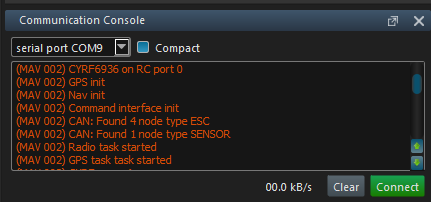
\includegraphics[width=0.5\textwidth]{graphics/test_register_node.png}
    \caption{Successful SENSOR registration}
    \label{fig:successful_register}
\end{figure}

\subsubsection*{Spoofed current test}
When an AQ PDB is mounted on a drone, the PDB measures voltage, current and temperature and sends the measurements to AQ where they get logged.\\
The code in section \ref{sec:reg_node_test} was further developed into a sensor simulator that spoofs current measurements into AQ to test the registering works probably. \\
A logger extension-board was mounted on the M4-board in order to save the measurements to a MicroSD-card.

Code \ref{code:spoof_current} shows the implementation where a sinus is generated to simulate a current and how it is transmitted to AQ. \cite{someguy2993}

\begin{lstlisting}[language = python, caption = Snippet spoofing current measurements into AQ, label=code:spoof_current]
def ReqistrerTelem(self):
	# self.sinus is a list of sinus values
	sensor_value = self.sinus[self.phase]

	# Get next value next time and do overrun
	self.phase+=1
	self.phase = self.phase % 20

	# Pack as IEEE754 float
	sensor_value_float = pack('>f', sensor_value)

	# Create list of float-bytes as integers
	data_float = [int(ord(elm)) for elm in sensor_value_float]

	# Reverse list and append empty data
	data_float.reverse()
	
	# Send to AQ. id =  CAN_FID_TELEM (02c00000) | Sourceid 1 (00000800) | CAN_SENSORS_PDB_BATA (00004000)
	self.send(0x02c04800, data_float)
\end{lstlisting}

The method defined in code \ref{code:spoof_current} was run every 100ms.\\
After the code ran for a few seconds the SD card was plugged into a PC and QgroundStation configured to make a plot of the PDB\_CURRENT-field. The plot can be seen in figure \ref{fig:pdb_current_log} 


\begin{figure}[H]
    \center
    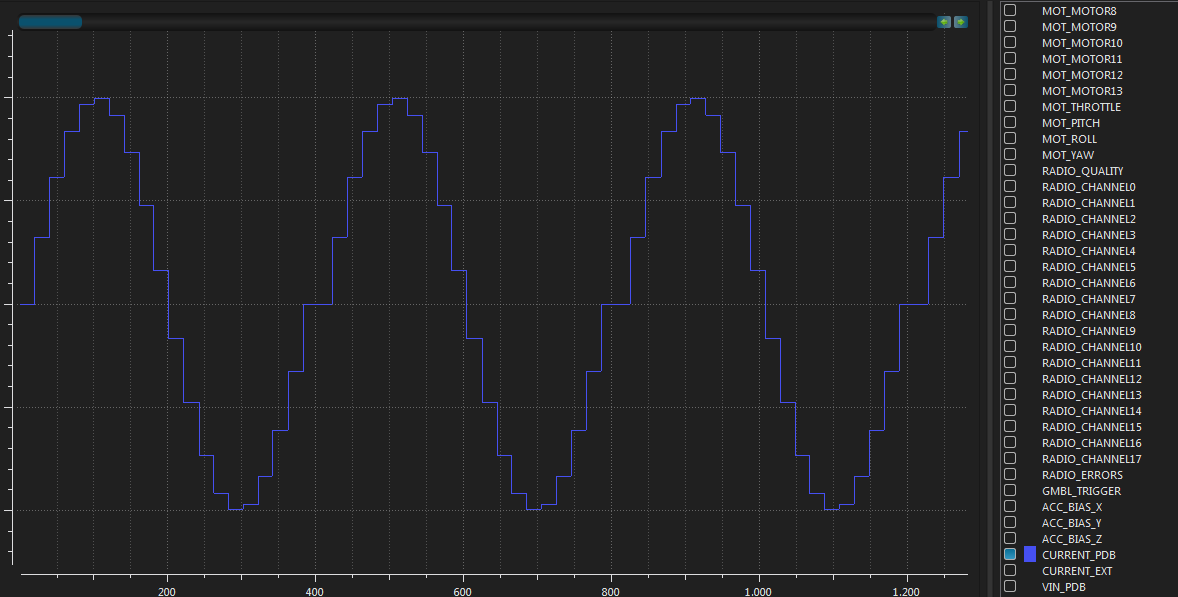
\includegraphics[width=0.8\textwidth]{graphics/test_can_spoof_current.png}
    \caption{Test of python CAN test}
    \label{fig:pdb_current_log}
\end{figure}

Figure \ref{fig:pdb_current_log} shows the sinus generated from the node as expected.

